\documentclass[5px]{report}
\usepackage{fullpage}
\usepackage{graphicx}
\usepackage[margin=0.25in]{geometry}

\begin{document}
\textbf{Authors}: Patrick O'Connell (oconne16) \& Jahnvi Patel (jpate201)
\begin{enumerate}
\item \textbf{What is your data and task (including data preprocessing steps)?} \\
Dataset for this project is acquired from \textit{Young People Survey} from \textit{kaggle.com}. The main task of the project is to predict a persons' empathy as either "very empathetic" or "not very empathetic". The dataset provided in the .csv files is either numerical or categorical. The numerical values were sorted based on 0 being the least and 5 being the most. While, the categorical data was sorted more delicately based on specific keywords (i.e. "never smoked" = 0, or "doctorate degree" = 5). The empty fields were filled with the total average of the column. After loading and cleaning up the data, we normalized the data so all the categories can have the same scale for a fair comparison between them. The people rated their empathy rate higher than 3 are marked as "very empathetic" while the rest are marked as "not very empathetic".

\item \textbf{What ML solution did you choose and, most importantly, why was this an appropriate choice?}\\
From the ML solutions we learned in class, we have chosen to implement K-Nearest Neighbors, Decision Tree, Gradient Descent using Loss functions (Hinge, Logistic, Squared) and Random Forest. We chose KNN due to its ability to pattern match, text mining and natural language processing. Decision Trees are great for classification and regression. The Loss functions are useful for mapping an event or values of variables onto a real number, which intuitively represents the "cost" associated with the event. Random Forest (RF) is an ensemble method, in which its classifiers provide higher accuracy and prevent overfitting (when more trees are present). The main principle of RF is that a group of "weak learners" can come together to form a "strong learner". In other words, each classifier, individually, is a "weak learner" while all the classifiers taken together create a "strong learner".

We used these algorithms to evaluate which algorithm would run the best against the baseline. Ultimately, Random Forest gave us the best resulting test accuracy of 79\% (approximately 15\% better than the baseline)

\item \textbf{How did you choose to evaluate success, including baselines, experimental setup (e.g., \% train/dev/test), metrics?}\\
In order to set up the experiments, the dataset is separated into training, validation and testing dataset. These were chosen based on rule-of-thumb (80-10-10) discussed in class . Given 1010 responses, 810 were chosen as training data, 100 were chosen as validation data and the remaining 100 responses were set aside as test data. Success of the algorithm is based on its performance compared to the baseline collected. If the algorithm performs better than the baseline accuracy then it is marked as a success.
The baseline is computed by using the training dataset marked with "very empathetic" and "not very empathetic" responses. Next, by using this training models most frequent empathetic state for out guessing strategy on the testing data, we obtain an accuracy of about 64\%.

\item \textbf{What software did you use and why did you choose it?}
  \begin{enumerate}
     \item matplotlib.pyplot: To visualize plots
     \item sklearn.tree: Classify decision tree-based models for classification and regression.
     \item sklearn.metrics: To compute score functions, performance metrics and pairwise metrics and distance computations.
 \end{enumerate}

\item \textbf{What are the results?}
\begin{figure}[h]
  \centering
  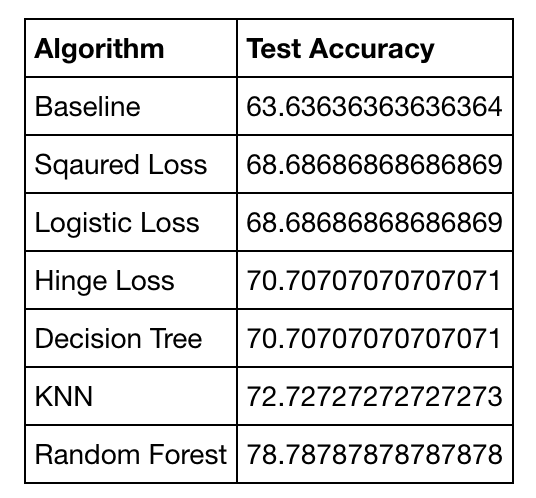
\includegraphics[height=1.25in]{results.png}
  \caption{Testing Accuracy of "empathetic" vs "not very empathetic"}
  \label{f:myplotfig}
\end{figure}

\item \textbf{Show some examples from the development data that your approach got correct and some it got wrong: if you were to try to fix the ones it got wrong, what would you do?}
The keys to understanding the faults in the predictions development data for the approaches that we used lies mostly with the tuning of hyperparameters.  This is to say that the development data exposed whether or not we were likely to be overfitting and underfitting our data for the various models that we used.  When it came to the decision tree classifier, we found that using depths greater that 6 would greatly overfit the training data and cause adverse effects when it came to the development accuracy.   The decision tree classifier actually saw accuracies below that of the baseline classifier when the depth was increase to 8 or greater.  However, larger maximum depths were permissible when using the Random Forest approach.  Here, overfitting seemed to occur past depths of around 50 but this was highly subject to the random fluctuations in the model itself.
\end{enumerate}
\end{document} 